\documentclass{standalone}
\usepackage{tikz}
\usetikzlibrary{arrows.meta}
\begin{document}
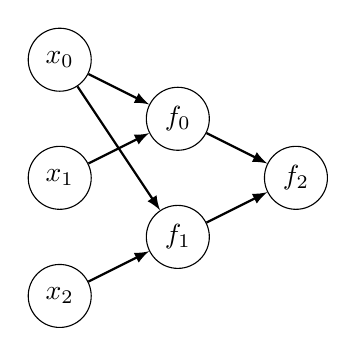
\begin{tikzpicture}[]

\begin{scope}[every node/.style={circle, draw, minimum size=8mm}]
    \node (x0) at (0, 0) {$x_0$};
    \node (x1) at (0,-1.5) {$x_1$};
    \node (x2) at (0,-3) {$x_2$};
    \node (a3) at (1.5,-0.75)  {$f_0$};
    \node (a4) at (1.5,-2.25) {$f_1$};
    \node (a5) at (3,-1.5) {$f_2$};
\end{scope}

\begin{scope}[-latex, thick]
    \draw (x0) -- (a3);
    \draw (x0) -- (a4);
    \draw (x1) -- (a3);
    \draw (x2) -- (a4);
    \draw (a3) -- (a5);
    \draw (a4) -- (a5);
\end{scope}

\end{tikzpicture}
\end{document}
